\documentclass{article} % For LaTeX2e
\usepackage{iclr2026_conference,times}
% NOTE: targeting ICLR 2027; using the iclr2026 style files until the 2027
% template is released (swap iclr2026_conference.{sty,bst} then).

% Optional math commands from https://github.com/goodfeli/dlbook_notation.
\input{math_commands.tex}

\usepackage{hyperref}
\usepackage{url}
\usepackage{graphicx}
\usepackage{textcomp}
%
% These are recommended to typeset algorithms but not required.
\usepackage{algorithm}
\usepackage{algorithmic}
%
% Recommended for better-looking tables
\usepackage{booktabs}
%
% For the capability comparison table (Table 1)
\usepackage{tikz}
\usepackage{adjustbox}
\usepackage{multirow}
%
% Math symbols
\usepackage{amsmath,amssymb}
%
% Colors for delta annotations in Table 2 (MAS rows vs LLM base).
\usepackage{xcolor}
\definecolor{deltaPos}{HTML}{006400}
\definecolor{deltaNeg}{HTML}{8B0000}
\definecolor{deltaTie}{HTML}{707070}
% \deltaup{x.x} / \deltadn{x.x} / \deltatie{0.0}
\newcommand{\deltaup}[1]{{\scriptsize\textcolor{deltaPos}{(\textuparrow #1)}}}
\newcommand{\deltadn}[1]{{\scriptsize\textcolor{deltaNeg}{(\textdownarrow #1)}}}
\newcommand{\deltatie}[1]{{\scriptsize\textcolor{deltaTie}{(#1)}}}
%
% For inline drafting notes; remove before camera-ready.
\usepackage[colorinlistoftodos,prependcaption,textsize=footnotesize]{todonotes}

\title{ARMOR: Adaptively Recursive Multi-agent ORchestration via Reinforcement Learning}

% Authors must not appear in the submitted version. They should be hidden
% as long as the \iclrfinalcopy macro remains commented out below.
\author{Anonymous authors}

%\iclrfinalcopy % Uncomment for camera-ready version, but NOT for submission.

\begin{document}

\maketitle

\begin{abstract}
% TODO: one paragraph. ICLR has no hard word limit but keep it concise.
\end{abstract}

\section{Introduction}
\label{sec:intro}

LLM-based multi-agent systems (MAS) have emerged as a powerful paradigm for
complex, real-world tasks that exceed the capacity of any single large language model (LLM)~\citep{%
fourney2024magentic,wang2025mas2,zhang2026metaagentx}.
The central advantage of MAS lies in specialization: by decomposing a complex
task into distinct subtasks and assigning each to a dedicated agent, the system
allows every agent to apply focused expertise within a narrowly scoped context,
reducing per-subtask error accumulation and improving overall
reliability~\citep{wang2025mas2,lin2024think}.
MAS have demonstrated performance advantages over single-agent
systems (SAS) across diverse and challenging domains.\todo{Specify application domains and add citations after benchmark selection.}
The development of MAS has fundamentally progressed along two axes:
the system-level orchestration of agents and the method-level optimization strategy.

At the system level, progress has centered on topological dynamics.
\emph{Manually static} systems prescribe a fixed topology through human
design~\citep{fourney2024magentic,chen2023autoagents}; \emph{automatically
static} systems instead generate a query-tailored topology before execution
begins~\citep{zhuge2024gptswarm,zhang2024gdesigner,gao2025flowreasoner,%
nielsen2026conductor,zhang2026metaagentx}.
\emph{Semi-dynamic} systems allow topology revision between runs but keep it
fixed within a single
execution~\citep{chen2024agentverse,hu2025evomac,wang2026metagen,%
wang2026agentconductor,wang2025mas2}.
\emph{Dynamic} systems go further, adapting topology within a single execution
as the task unfolds~\citep{dang2026multi,jiang2026agentqmix,wang2025tdag}.
Yet across all four generations, topology is determined by heuristic rules rather
than learned from task outcomes, imposing a hard ceiling: performance is confined
to what human initialization can anticipate~\citep{hu2025evomac}, and optimal
coordination structures can only emerge through reward-driven learning,
not upfront design~\citep{nielsen2026conductor}.

At the method level, training strategies have advanced from
hand-crafted heuristic coordination rules~\citep{fourney2024magentic,%
chen2023autoagents}, to lightweight routing modules trained with the backbone
LLM frozen~\citep{zhuge2024gptswarm,zhang2024gdesigner,jiang2026agentqmix,%
dang2026multi}, to end-to-end RL fine-tuning of the backbone LLM
itself~\citep{zhang2026metaagentx,nielsen2026conductor,gao2025flowreasoner,%
wang2025mas2}.
Yet all three prioritize designing the right orchestration of agents in advance,
not adapting it as execution unfolds.
This \emph{generate-once-and-deploy} assumption is brittle: any
unforeseen disruption during execution, such as a tool failure, an unexpected
subtask outcome, or a mid-task shift in difficulty, can cascade into system-wide
failure, as the orchestration of agents has no capacity to adapt beyond its
initial instantiation~\citep{wang2025mas2}.

To address these limitations, we propose \textbf{ARMOR}, an \textbf{A}daptively \textbf{R}ecursive \textbf{M}ulti-agent \textbf{OR}chestration framework trained end-to-end via
reinforcement learning.
Every agent runs the same learned policy: it may execute its assigned
task directly, or orchestrate a team of sub-agents to handle it.
As any agent in the execution graph may itself become an orchestrator,
our framework is recursive and the topology is inherently dynamic.
Training ARMOR end-to-end via reinforcement learning yields three emergent
properties: a task-conditioned dynamic \emph{topology} that distributes context load
evenly across agents, preventing any single agent from becoming a context
bottleneck\todo{Analysis: measure per-agent peak context load; show
RL-learned topology achieves more balanced load distribution than heuristic
baselines.}; agent \emph{roles} that span the full natural language role space,
unconstrained by any fixed pool; and fine-grained \emph{content} management that shields each agent from
task-irrelevant context, improving the reliability of specialized subtask
execution.
All three properties are calibrated to the actual capabilities of the
underlying LLM, rather than to the assumptions of human designers.

\todo[inline]{Para 5: results + contributions.}

\begin{figure}[t]
    \centering
    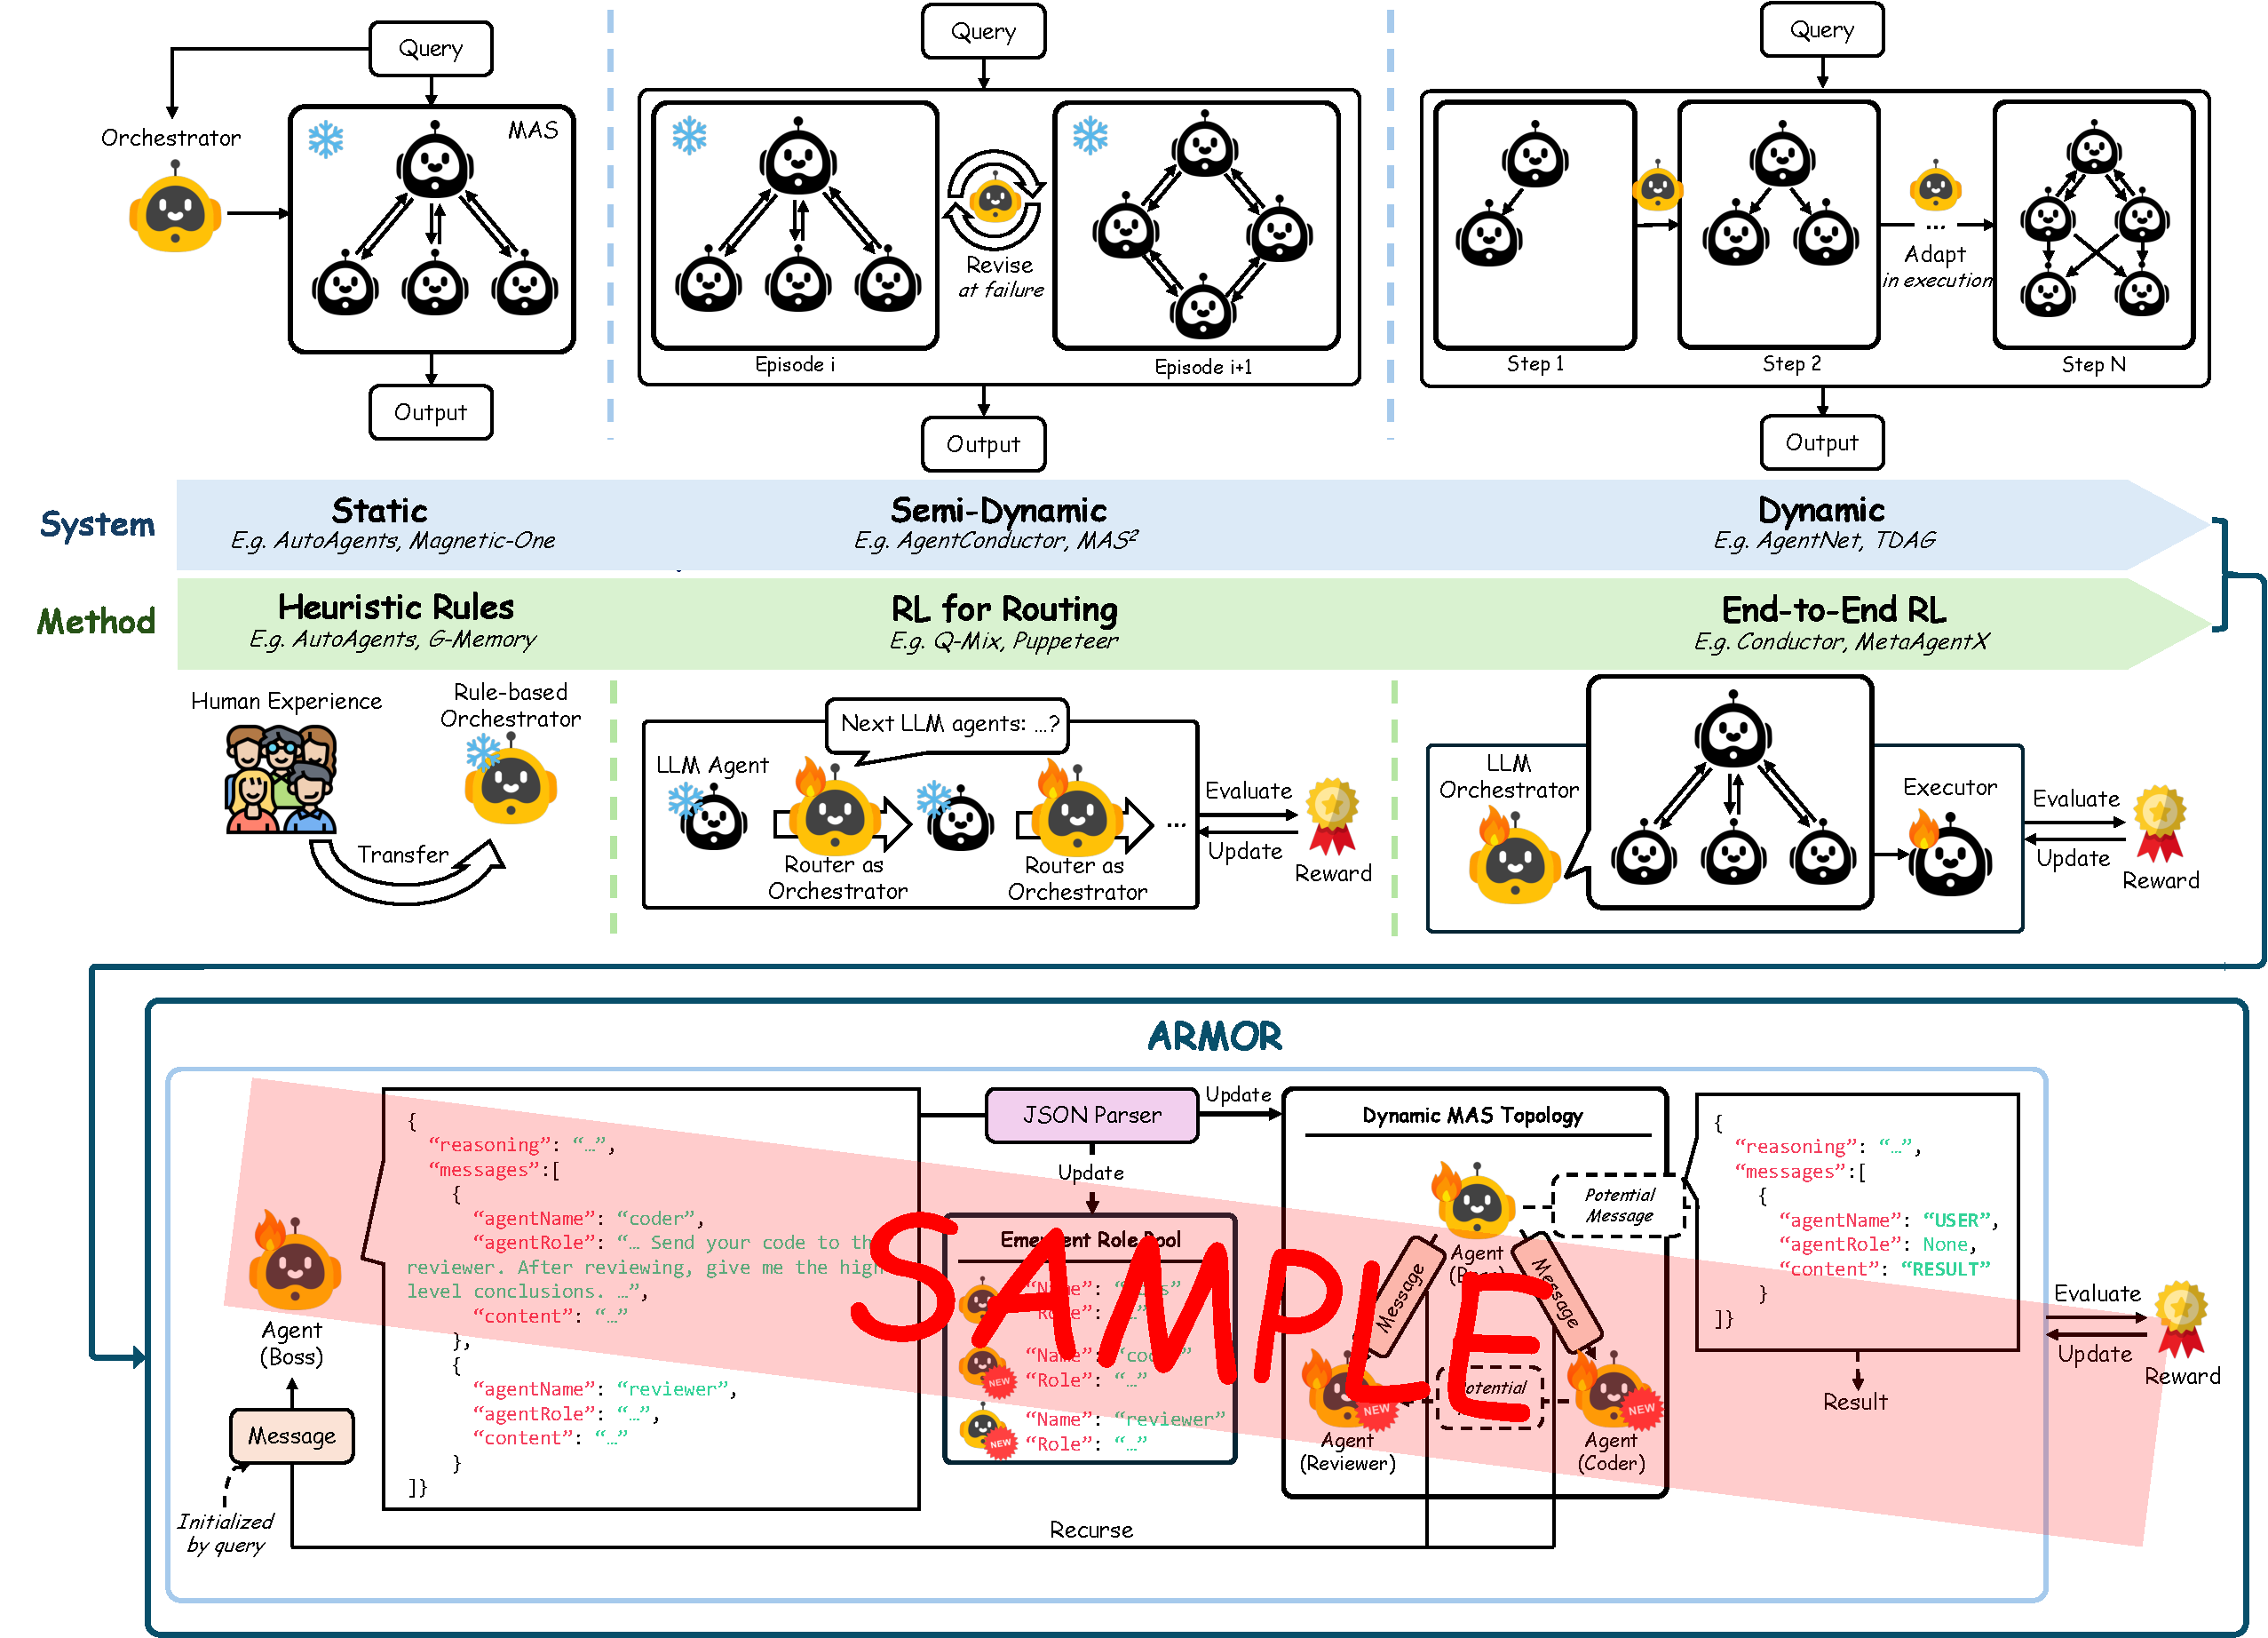
\includegraphics[width=\textwidth]{Figures/teaser.pdf}
    \caption{Overview of ARMOR.}
    \label{fig:teaser}
\end{figure}

\section{Related Work}

\todo[inline]{Related Work is a funnel narrowing to our gap. Two subsections: (1) single-agent memory is mature but assumes a single reader/writer, so it has no content management; (2) multi-agent systems surface that layer; we organize them by \emph{when} the topology can change---Static (fixed before execution), Semi-dynamic (fixed within a run, revised across runs), and Dynamic (adapts during execution)---each subdividing into heuristic vs.\ RL-learned. Across all of them, adaptation governs message routing over preset or generated roles only; none governs which memory content an agent may access or how writes are verified and reconciled, and none uses RL to let roles emerge from such a policy. That empty cell is us.}

% --- Harvey-ball badges for Table~\ref{tab:comparison} (full/half/empty = strong/partial/none) ---
\newcommand{\capG}{\tikz[baseline=-0.55ex]{\filldraw[green!55!black] (0,0) circle (0.4em);}}
\newcommand{\capM}{\tikz[baseline=-0.55ex]{\draw[orange!90!black,line width=0.4pt] (0,0) circle (0.4em);\fill[orange!90!black] (0,-0.4em) arc (-90:90:0.4em) -- cycle;}}
\newcommand{\capB}{\tikz[baseline=-0.55ex]{\draw[red!80,line width=0.4pt] (0,0) circle (0.4em);}}

\begin{table}[t]
\centering
\small
\begin{adjustbox}{max width=\columnwidth}
\begin{tabular}{lccc|c}
\toprule
\textbf{Framework} & \textbf{Topology} & \textbf{Role} & \textbf{Content} & \textbf{Train} \\
\midrule
Magentic-One~\citep{fourney2024magentic} & \capB & \capB & \capB & \capB \\
AutoAgents~\citep{chen2023autoagents} & \capB & \capG & \capM & \capB \\
G-Memory~\citep{zhang2025gmemory} & \capB & \capB & \capM & \capB \\
TDAG~\citep{wang2025tdag} & \capG & \capG & \capG & \capB \\
\midrule
MetaGen~\citep{wang2026metagen} & \capM & \capG & \capG & \capM \\
AgentNet~\citep{yang2025agentnet} & \capG & \capG & \capG & \capM \\
GPTSwarm~\citep{zhuge2024gptswarm} & \capB & \capB & \capG & \capM \\
G-Designer~\citep{zhang2024gdesigner} & \capB & \capB & \capG & \capM \\
Agent Q-Mix~\citep{jiang2026agentqmix} & \capG & \capB & \capM & \capM \\
Puppeteer~\citep{dang2026multi} & \capG & \capB & \capB & \capM \\
\midrule
FlowReasoner~\citep{gao2025flowreasoner} & \capM & \capG & \capG & \capG \\
AgentConductor~\citep{wang2026agentconductor} & \capM & \capB & \capG & \capG \\
MAS$^2$~\citep{wang2025mas2} & \capM & \capG & \capG & \capG \\
Conductor~\citep{nielsen2026conductor} & \capB & \capG & \capG & \capG \\
MetaAgent-X~\citep{zhang2026metaagentx} & \capB & \capG & \capG & \capG \\
\textbf{ARMOR (Ours)} & \capG & \capG & \capG & \capG \\
\bottomrule
\end{tabular}
\end{adjustbox}
\caption{Capability comparison of representative multi-agent frameworks. Each dimension is rated with a full / half / empty circle. The first three columns are system-level (how the system is organized); \emph{Train} (right of the rule) is method-level (how it is optimized). \emph{Topology}: dynamic / semi-dynamic / static. \emph{Role}: emergent, i.e., created by the system (generated per task or learned) / fixed, i.e., a hand-designed pool. \emph{Content}: whether agents see differentiated, duty-focused parts of the task context -- full isolation, i.e., each agent sees only its assigned part (via curated context, code-level dataflow, or restricted message passing) / partial differentiation without strict isolation (e.g., retrieval- or summary-based filtering) / one shared context for all agents. \emph{Train}: what is trained -- the backbone LLM itself / auxiliary parameters outside the frozen LLM, ranging from lightweight edge weights or scoring priors to routers and value networks / nothing, i.e., an off-the-shelf LLM works plug-and-play.}
\label{tab:comparison}
\end{table}

\subsection{Single-Agent System (SAS)}
\todo[inline]{Goal: establish the starting point and the gap, NOT a literature dump. Briefly survey SAS memory (e.g., MemGPT, MemTree, GraphRAG): storage, compression, retrieval are well studied. Then make the pivot: SAS methods all assume a \emph{single reader/writer}, so they have no notion of \emph{content management} -- who may see what, whose write is trustworthy, how to reconcile conflicting writes, how to isolate noise. Moving from SAS to MAS introduces this entire layer. One-sentence transition into the next subsection.}

\subsection{Multi-Agent System (MAS)}

A multi-agent system (MAS) coordinates multiple LLM-based agents through a communication topology to solve tasks beyond a single agent's reach. We organize MAS into three classes according to when they can adapt the topology: static, semi-dynamic, and dynamic.

\paragraph{Static}
Static MAS fix the topology at query time and do not reorganize it as the task unfolds. Notably, the distinction concerns the topology, not agent-internal functionality, so systems that keep it fixed while only adapting agent roles or behavior~\citep{xue2026comas,peng2026sage,lu2024morphagent} are still considered static. Neither does scheduling count: when a hand-designed control loop merely selects which member of a fixed team acts next, while every message still flows through the same hub structure, the communication structure itself never changes.
Their topology is centralized around a single orchestrator~\citep{fourney2024magentic,chen2023autoagents}, decentralized with peer-to-peer agents~\citep{hao2026decentmem,zhuge2024gptswarm}, or hybrid, generating the topology per query and then freezing it before execution. Such generators are produced in three ways: prompting an LLM in context~\citep{lin2024think}, training a lightweight router or graph designer while keeping the backbone LLM frozen~\citep{yue2025masrouter,zhang2024gdesigner}, or fine-tuning the LLM itself end-to-end with RL~\citep{nielsen2026conductor,zhang2026metaagentx}.

\paragraph{Semi-dynamic}
Semi-dynamic MAS keep the topology fixed within a single execution but revise it across executions, e.g., re-recruiting the team on failure~\citep{chen2024agentverse}, iteratively refining roles and connections~\citep{hu2025evomac,wang2026metagen}, reflecting after the task~\citep{hao2026evolve}, or training a policy to regenerate the topology~\citep{wang2026agentconductor,wang2025mas2,gao2025flowreasoner}.

\paragraph{Dynamic}
Dynamic MAS reorganize the topology during a single execution, as the task unfolds.
Heuristically dynamic MAS follow fixed rules, e.g., pruning low-contribution agents mid-run by peer rating~\citep{liu2023dynamic}, spawning sub-agents on demand to match complexity~\citep{wang2025megaagent,ishibashi2024self}, hiring and firing workers in real time~\citep{lyu2026self}, or routing a query through a pre-trained graph or state machine~\citep{yang2025agentnet,zhang2025metaagent}.
Learning-based dynamic MAS, a still under-explored direction, instead train a policy that updates the topology step by step, e.g., composing a serialized chain of agents whose outputs feed one another~\citep{dang2026multi}, composing it from per-agent communication actions~\citep{jiang2026agentqmix}, rerouting around unreliable agents~\citep{fan2026todycomm}, or selecting a stage-specific workflow as execution unfolds~\citep{xu2026evomas,wang2026mango}.
\todo[inline]{One-sentence closing (placeholder): position our gap as an RL-learned policy over memory-content access and write governance, from which roles emerge; forward-reference Method.}

\section{Method}

\subsection{Problem Definition}

We model a multi-agent system (MAS) as a set of LLM agents that communicate
through a shared message queue to collectively solve a task $q$ issued by a user.

\paragraph{Agents, profiles, and memory}
Let $\mathcal{A}^t$ denote the set of active agents at step $t$.
To coordinate effectively, agents must maintain awareness of their teammates'
capabilities and current state without accessing each other's full execution histories.
Each agent $i \in \mathcal{A}^t$ therefore maintains a \emph{profile}
$\rho_i^t$, a compressed, public-facing natural-language document encoding its name,
current responsibilities, and a running summary of past actions.
The \emph{team roster} $\mathcal{T}^t = \{(i,\,\rho_i^t)\}_{i \in \mathcal{A}^t}$
is globally visible to every agent but can only be written by its owner:
agent $i$ may update $\rho_i$ but not $\rho_j$ for $j \neq i$.
The \emph{memory} $\mathcal{M}_i^t$, by contrast, is a private, lossless record
for the agent itself: a chronological log of every prior activation of agent $i$,
comprising the incoming message, the reasoning trace, the outgoing messages,
and the resulting profile update.

\paragraph{Messages}
A message $m = (s, r, c)$ consists of a sender $s$, a recipient $r$, and
natural-language content $c$,
where $s, r \in \mathcal{A}^t \cup \{\texttt{user}\}$.
Trivial fields that are determined by context are excluded from the agent's
input and output: for example, when agent $i$ is activated, the recipient
satisfies $r = i$ by definition and is therefore not included in the agent's input.

\paragraph{Shared policy}
All agents execute a single shared policy $\pi_\theta$.
Agents are differentiated not by separate parameters but solely by their
inputs: the incoming message, the team roster, and the private memory.
When agent $i$ is activated with incoming message $m_i^t = (s, i, c)$, the policy
produces a single auto-regressive output sequence:
\begin{equation}
    (z_i^t,\;\mathbf{o}_i^t,\;\rho_i^{t+1})
    \;=\;
    \pi_\theta\!\left(m_i^t,\;\mathcal{T}^t,\;\mathcal{M}_i^t\right),
    \label{eq:policy}
\end{equation}
where $z_i^t$ is a \emph{reasoning trace},
$\mathbf{o}_i^t = [(i,r_1,c_1),\ldots,(i,r_k,c_k)]$ is a list of outgoing messages,
and $\rho_i^{t+1}$ is the agent's self-updated profile.
% The reasoning trace $z_i^t$ is also appended to $\mathcal{M}_i^{t+1}$,
% making it part of the agent's persistent memory.
\todo{Decide: should $z_i^t$ be stored in $\mathcal{M}_i$? Putting reasoning in memory enables self-reflection but increases context load.}

\paragraph{Execution}
The system maintains a FIFO message queue $\mathcal{Q}$.
Execution is initialized with a single entry-point agent $a_0$,
empty memory, and the user's query enqueued as the first message:
$\mathcal{A}^0 = \{a_0\}$, $\mathcal{Q}^0 = [(\texttt{user},\,q)]$.
At each step $t$:
\begin{enumerate}
    \item Dequeue the front message $(s, r, c)$ from $\mathcal{Q}^t$.
    \item If $r \notin \mathcal{A}^t$, \emph{spawn} agent $r$:
          add $r$ to $\mathcal{A}^t$ with empty memory and a blank profile.
          Spawning is implicit: it requires no special action type,
          and the spawning message itself serves as the new agent's first briefing.
    \item Activate agent $r$ via Eq.~\ref{eq:policy};
          update $\rho_r$ and $\mathcal{M}_r$ accordingly.
    \item Enqueue each $(r,\,r_j,\,c_j) \in \mathbf{o}_r^t$ into $\mathcal{Q}^{t+1}$.
\end{enumerate}
Execution terminates when an outgoing message with $r_j = \texttt{user}$
is produced (the final answer delivered to the user), or when the step
count reaches a budget $T$. If the budget is exhausted without any message
reaching the user, the execution is treated as a failure.

\paragraph{Learning objective}
Let $e = \bigl(m^0, z^0, \mathbf{o}^0,\,\ldots,\,m^\tau, z^\tau, \mathbf{o}^\tau\bigr)$
denote the full execution trajectory, where $\tau \leq T$ is the termination step.
Given a task reward $R(q, e) \in [0,1]$ reflecting answer correctness,
the learning objective is:
\begin{equation}
    \max_\theta\;\mathbb{E}_{q \sim \mathcal{D}}\bigl[R(q,\,e)\bigr],
    \label{eq:objective}
\end{equation}
where $\mathcal{D}$ is the task distribution and $e$ is the trajectory
induced by $\pi_\theta$ on query $q$.

\paragraph{Remark}
This formulation directly grounds the emergent properties introduced in the Introduction.
First, topology is never fixed in advance: at each step, $\pi_\theta$ decides
whom to message based on the current task state, and new agents are spawned
on demand, so the communication graph evolves throughout execution.
Second, roles are not predefined: specialization emerges from the combined
effect of message routing decisions, in-context reasoning, and self-maintained
profiles, with the profile serving as the explicit, readable record of an agent's
emerged identity.
Third, content is managed both structurally and behaviorally: each agent's
memory is private by construction, and through RL the policy learns what to
communicate and what to withhold, rather than forwarding raw execution details
indiscriminately.

\subsection{Supervised Fine-Tuning (SFT)}

\paragraph{Data collection}

\begin{table}[t]
\centering
\small
\begin{adjustbox}{max width=\textwidth}
\begin{tabular}{ll|cccc|ccc|cc|c|c}
\toprule
 & & \multicolumn{4}{c|}{\textbf{Math}} & \multicolumn{3}{c|}{\textbf{Code}} & \multicolumn{2}{c|}{\textbf{Multi-hop QA}} & \textbf{Science} & \textbf{Assistant} \\
\cmidrule(lr){3-6}\cmidrule(lr){7-9}\cmidrule(lr){10-11}\cmidrule(lr){12-12}\cmidrule(lr){13-13}
\textbf{Type} & \multicolumn{1}{c|}{\textbf{Collector}} & AIME-past & MATH & DAPO & Polaris & LCB & APPS & CC & HotpotQA & MuSiQue & GPQA & GAIA \\
\midrule
\multirow{3}{*}{Single-agent}
 & Llama-3.2-3B & 14.0 & 63.2 & 11.3 & 11.3 & 10.8 & 4.9 & 6.8 & 47.5 & 23.1 & 28.5 & 2.1 \\
 & Llama-3.1-8B & 11.6 & 66.4 & 12.2 & 11.2 & 16.6 & 5.5 & 10.1 & 58.5 & 38.9 & 31.5 & 2.7 \\
 & Qwen3-8B & 38.6 & 83.8 & 49.1 & 37.2 & 51.6 & 8.0 & 25.8 & 65.4 & 48.5 & 43.1 & 5.1 \\
\midrule
\multirow{3}{*}{Multi-agent}
 & MetaAgent-X~\citep{zhang2026metaagentx} & 46.3 & 80.4 & 10.1 & 39.2 & 38.2 & 45.1 & 19.4 & 18.8 & 33.9 & 41.1 & 4.8 \\
 & MetaAgent-X (no-tool)~\citep{zhang2026metaagentx} & 34.3 & 51.1 & 43.0 & 21.4 & -- & -- & -- & 31.5 & 15.8 & 37.4 & 5.6 \\
 & MetaAgent-X (reported)$^\dagger$~\citep{zhang2026metaagentx} & -- & -- & -- & -- & 41.0 & 38.0 & 17.0 & -- & -- & -- & -- \\
\bottomrule
\end{tabular}
\end{adjustbox}
\caption{Training-set trajectory success rate (pass@1, \%) of single-agent vs.\ multi-agent
collectors---a property of our SFT data, \emph{not} a main result. pass@1 is the fraction of
collected trajectories that are correct. Single-agent: each base LLM answers in one pass with no
scaffold and no tools ($n{=}4$ samples/problem, temperature $0.8$; Qwen3-8B with thinking
disabled). Multi-agent: MetaAgent-X's
shared designer+executor checkpoint ($n{=}1$ sample/problem; the \emph{no-tool} variant disables
external tools and does not collect code). ``--'' marks a domain a collector did not cover.
\emph{Math} scored by boxed answer + symbolic verification; \emph{Code} by sandboxed unit tests;
\emph{Multi-hop QA} by exact match over a step-by-step answer; \emph{GPQA} by letter match;
\emph{GAIA} by the official scorer. AIME-past/MATH/DAPO/Polaris and LCB(-v1)/APPS/CC(CodeContests)
are the training corpora (distinct from the Table~\ref{tab:main_results} test benchmarks).
$^\dagger$Numbers \emph{reported} in the MetaAgent-X paper (RL, Qwen3-8B), shown only for the
LCB/APPS/CC benchmarks that match a column; their test-set accuracy is not directly comparable to
the training-set pass@1 of the other rows. Their reported AIME24/AIME25/OlympiadBench
($40.0/33.3/61.0$) have no matching training column and are omitted.}
\label{tab:sft_data_success}
\end{table}

\paragraph{Data augmentation}

\subsection{Reinforcement Learning (RL)}


\section{Experiments}

\subsection{Experimental Setup}

\paragraph{Tasks and benchmarks}

\paragraph{Baselines}

\paragraph{Models}

\paragraph{Implementation details}

\subsection{Main Results}

\begin{table}[t]
\centering
\small
\begin{adjustbox}{max width=\textwidth}
\begin{tabular}{cl|ccc|ccc|cc|c|c}
\toprule
\multicolumn{1}{c}{\multirow{2}{*}{\textbf{Type}}} & \multicolumn{1}{c|}{\multirow{2}{*}{\textbf{Method}}} & \multicolumn{3}{c|}{\textbf{Math}} & \multicolumn{3}{c|}{\textbf{Code}} & \multicolumn{2}{c|}{\textbf{Multi-hop QA}} & \textbf{Science} & \textbf{Assistant} \\
\cmidrule(lr){3-5}\cmidrule(lr){6-8}\cmidrule(lr){9-10}\cmidrule(lr){11-11}\cmidrule(lr){12-12}
 & & MATH500 & AIME24 & AIME25 & LCB & APPS & CC & HotpotQA & MuSiQue & GPQA & GAIA \\
\midrule
\multirow{6}{*}{Base}
 & LLM-only (Llama-3.2-3B) & 53.0 & 10.0 & 0.0 & 12.6 & 7.3 & 1.8 & 50.0 & 18.7 & 27.3 & 4.5 \\
 & LLM-only (Llama-3.1-8B) & 55.0 & 10.0 & 0.0 & 16.0 & 8.7 & 3.0 & 64.0 & 27.3 & 24.2 & 2.3 \\
 & LLM-only (Qwen3.5-4B)   & 92.0 & 56.7 & 33.3 & 32.6 & 37.3 & 20.0 & 69.3 & 36.0 & 74.2 & 6.8 \\
 & LLM-only (Qwen3.5-9B)   & 98.0 & 63.3 & 53.3 & 39.4 & 48.7 & 26.1 & 70.0 & 46.0 & 66.7 & 11.4 \\
 & SFT (w/o reasoning) & -- & -- & -- & -- & -- & -- & -- & -- & -- & -- \\
 & SFT (w/ reasoning)  & -- & -- & -- & -- & -- & -- & -- & -- & -- & -- \\
\midrule
SAS
 & -- & -- & -- & -- & -- & -- & -- & -- & -- & -- & -- \\
\midrule
\multirow{16}{*}{\shortstack{MAS\\(Heuristic)}}
 & TDAG (Llama-3.2-3B)~\citep{wang2025tdag} & 12.0\,\deltadn{41.0} & 6.7\,\deltadn{3.3} & 0.0\,\deltatie{0.0} & 2.3\,\deltadn{10.3} & 1.3\,\deltadn{6.0} & 0.0\,\deltadn{1.8} & 22.0\,\deltadn{28.0} & 7.3\,\deltadn{11.3} & 36.4\,\deltaup{9.1} & 0.0\,\deltadn{4.5} \\
 & TDAG (Llama-3.1-8B)~\citep{wang2025tdag} & 20.0\,\deltadn{35.0} & 6.7\,\deltadn{3.3} & 0.0\,\deltatie{0.0} & 14.9\,\deltadn{1.1} & 10.7\,\deltaup{2.0} & 3.6\,\deltaup{0.6} & 33.3\,\deltadn{30.7} & 16.0\,\deltadn{11.3} & 33.3\,\deltaup{9.1} & 2.3\,\deltatie{0.0} \\
 & TDAG (Qwen3.5-4B)~\citep{wang2025tdag} & 89.0\,\deltadn{3.0} & 50.0\,\deltadn{6.7} & 40.0\,\deltaup{6.7} & 17.1\,\deltadn{15.4} & 19.3\,\deltadn{18.0} & 10.3\,\deltadn{9.7} & 73.3\,\deltaup{4.0} & 57.3\,\deltaup{21.3} & 69.7\,\deltadn{4.5} & 9.1\,\deltaup{2.3} \\
 & TDAG (Qwen3.5-9B)~\citep{wang2025tdag} & 89.0\,\deltadn{9.0} & 36.7\,\deltadn{26.7} & 30.0\,\deltadn{23.3} & 30.9\,\deltadn{8.6} & 32.0\,\deltadn{16.7} & 18.8\,\deltadn{7.3} & 66.0\,\deltadn{4.0} & 38.7\,\deltadn{7.3} & 74.2\,\deltaup{7.6} & 13.6\,\deltaup{2.3} \\
 & AutoAgents (Llama-3.2-3B)~\citep{chen2023autoagents} & 25.0\,\deltadn{28.0} & 0.0\,\deltadn{10.0} & 0.0\,\deltatie{0.0} & 5.7\,\deltadn{6.9} & 6.7\,\deltadn{0.7} & 0.6\,\deltadn{1.2} & 23.3\,\deltadn{26.7} & 18.7\,\deltatie{0.0} & 33.3\,\deltaup{6.1} & 2.3\,\deltadn{2.3} \\
 & AutoAgents (Llama-3.1-8B)~\citep{chen2023autoagents} & 31.0\,\deltadn{24.0} & 3.3\,\deltadn{6.7} & 0.0\,\deltatie{0.0} & 4.0\,\deltadn{12.0} & 0.7\,\deltadn{8.0} & 0.0\,\deltadn{3.0} & 31.3\,\deltadn{32.7} & 18.0\,\deltadn{9.3} & 36.4\,\deltaup{12.1} & 6.8\,\deltaup{4.5} \\
 & AutoAgents (Qwen3.5-4B)~\citep{chen2023autoagents} & 84.0\,\deltadn{8.0} & 36.7\,\deltadn{20.0} & 36.7\,\deltaup{3.3} & 13.1\,\deltadn{19.4} & 13.3\,\deltadn{24.0} & 9.7\,\deltadn{10.3} & 68.7\,\deltadn{0.7} & 40.0\,\deltaup{4.0} & 48.5\,\deltadn{25.8} & 6.8\,\deltatie{0.0} \\
 & AutoAgents (Qwen3.5-9B)~\citep{chen2023autoagents} & 84.0\,\deltadn{14.0} & 43.3\,\deltadn{20.0} & 33.3\,\deltadn{20.0} & 28.6\,\deltadn{10.9} & 32.7\,\deltadn{16.0} & 21.2\,\deltadn{4.8} & 74.0\,\deltaup{4.0} & 57.3\,\deltaup{11.3} & 71.2\,\deltaup{4.5} & 15.9\,\deltaup{4.5} \\
 & Magentic-One (Llama-3.2-3B)~\citep{fourney2024magentic} & 42.0\,\deltadn{11.0} & 3.3\,\deltadn{6.7} & 0.0\,\deltatie{0.0} & 9.1\,\deltadn{3.4} & 7.3\,\deltatie{0.0} & 4.2\,\deltaup{2.4} & 52.0\,\deltaup{2.0} & 17.3\,\deltadn{1.3} & 27.3\,\deltatie{0.0} & 0.0\,\deltadn{4.5} \\
 & Magentic-One (Llama-3.1-8B)~\citep{fourney2024magentic} & 50.0\,\deltadn{5.0} & 3.3\,\deltadn{6.7} & 0.0\,\deltatie{0.0} & 16.0\,\deltatie{0.0} & 8.7\,\deltatie{0.0} & 3.6\,\deltaup{0.6} & 60.0\,\deltadn{4.0} & 38.7\,\deltaup{11.3} & 30.3\,\deltaup{6.1} & 9.1\,\deltaup{6.8} \\
 & Magentic-One (Qwen3.5-4B)~\citep{fourney2024magentic} & 85.0\,\deltadn{7.0} & 33.3\,\deltadn{23.3} & 33.3\,\deltatie{0.0} & 36.0\,\deltaup{3.4} & 38.7\,\deltaup{1.3} & 13.9\,\deltadn{6.1} & 74.7\,\deltaup{5.3} & 53.3\,\deltaup{17.3} & 56.1\,\deltadn{18.2} & 13.6\,\deltaup{6.8} \\
 & Magentic-One (Qwen3.5-9B)~\citep{fourney2024magentic} & 86.0\,\deltadn{12.0} & 26.7\,\deltadn{36.7} & 16.7\,\deltadn{36.7} & 33.7\,\deltadn{5.7} & 30.7\,\deltadn{18.0} & 15.2\,\deltadn{10.9} & 76.7\,\deltaup{6.7} & 56.0\,\deltaup{10.0} & 77.3\,\deltaup{10.6} & 20.4\,\deltaup{9.1} \\
 & AgentNet (Llama-3.2-3B)~\citep{yang2025agentnet} & 43.0\,\deltadn{10.0} & 0.0\,\deltadn{10.0} & 0.0\,\deltatie{0.0} & 10.9\,\deltadn{1.7} & 6.7\,\deltadn{0.7} & 2.4\,\deltaup{0.6} & 47.3\,\deltadn{2.7} & 22.0\,\deltaup{3.3} & 24.2\,\deltadn{3.0} & 2.3\,\deltadn{2.3} \\
 & AgentNet (Llama-3.1-8B)~\citep{yang2025agentnet} & 43.0\,\deltadn{12.0} & 0.0\,\deltadn{10.0} & 0.0\,\deltatie{0.0} & 6.3\,\deltadn{9.7} & 6.7\,\deltadn{2.0} & 1.2\,\deltadn{1.8} & 48.7\,\deltadn{15.3} & 25.3\,\deltadn{2.0} & 18.2\,\deltadn{6.1} & 0.0\,\deltadn{2.3} \\
 & AgentNet (Qwen3.5-4B)~\citep{yang2025agentnet} & 94.0\,\deltaup{2.0} & 60.0\,\deltaup{3.3} & 36.7\,\deltaup{3.3} & 34.9\,\deltaup{2.3} & 36.0\,\deltadn{1.3} & 18.8\,\deltadn{1.2} & 77.3\,\deltaup{8.0} & 56.7\,\deltaup{20.7} & 77.3\,\deltaup{3.0} & 11.4\,\deltaup{4.5} \\
 & AgentNet (Qwen3.5-9B)~\citep{yang2025agentnet} & 97.0\,\deltadn{1.0} & 56.7\,\deltadn{6.7} & 36.7\,\deltadn{16.7} & 42.9\,\deltaup{3.4} & 46.0\,\deltadn{2.7} & 25.4\,\deltadn{0.6} & 75.3\,\deltaup{5.3} & 56.7\,\deltaup{10.7} & 75.8\,\deltaup{9.1} & 20.4\,\deltaup{9.1} \\
\midrule
\multirow{8}{*}{\shortstack{MAS\\(Routing RL)}}
 & Puppeteer (Llama-3.2-3B, per-domain)~\citep{dang2026multi} & 56.0\,\deltaup{3.0} & 3.3\,\deltadn{6.7} & 3.3\,\deltaup{3.3} & 12.0\,\deltadn{0.6} & 7.3\,\deltatie{0.0} & 2.4\,\deltaup{0.6} & 56.7\,\deltaup{6.7} & 22.0\,\deltaup{3.3} & 25.8\,\deltadn{1.5} & 4.5\,\deltatie{0.0} \\
 & Puppeteer (Llama-3.1-8B, per-domain)~\citep{dang2026multi} & 55.0\,\deltatie{0.0} & 3.3\,\deltadn{6.7} & 6.7\,\deltaup{6.7} & 17.1\,\deltaup{1.1} & 10.0\,\deltaup{1.3} & 4.2\,\deltaup{1.2} & 52.0\,\deltadn{12.0} & 28.7\,\deltaup{1.4} & 36.4\,\deltaup{12.2} & 2.3\,\deltatie{0.0} \\
 & Puppeteer (Qwen3.5-4B, per-domain)~\citep{dang2026multi} & 91.0\,\deltadn{1.0} & 50.0\,\deltadn{6.7} & 43.3\,\deltaup{10.0} & 34.3\,\deltaup{1.7} & 34.7\,\deltadn{2.6} & 17.0\,\deltadn{3.0} & 69.3\,\deltatie{0.0} & 44.7\,\deltaup{8.7} & 60.6\,\deltadn{13.6} & 6.8\,\deltatie{0.0} \\
 & Puppeteer (Qwen3.5-9B, per-domain)~\citep{dang2026multi} & 95.0\,\deltadn{3.0} & 66.7\,\deltaup{3.4} & 56.7\,\deltaup{3.4} & 40.0\,\deltaup{0.6} & 46.7\,\deltadn{2.0} & 22.4\,\deltadn{3.7} & 72.7\,\deltaup{2.7} & 52.0\,\deltaup{6.0} & 62.1\,\deltadn{4.6} & 9.1\,\deltadn{2.3} \\
 & Puppeteer (Llama-3.2-3B, shared)~\citep{dang2026multi} & 53.0\,\deltatie{0.0} & 0.0\,\deltadn{10.0} & 0.0\,\deltatie{0.0} & 8.6\,\deltadn{4.0} & 5.3\,\deltadn{2.0} & 3.6\,\deltaup{1.8} & 46.7\,\deltadn{3.3} & 21.3\,\deltaup{2.6} & 30.3\,\deltaup{3.0} & 2.3\,\deltadn{2.2} \\
 & Puppeteer (Llama-3.1-8B, shared)~\citep{dang2026multi} & 61.0\,\deltaup{6.0} & 13.3\,\deltaup{3.3} & 6.7\,\deltaup{6.7} & 17.1\,\deltaup{1.1} & 11.3\,\deltaup{2.6} & 3.0\,\deltatie{0.0} & 61.3\,\deltadn{2.7} & 40.7\,\deltaup{13.4} & 34.8\,\deltaup{10.6} & 2.3\,\deltatie{0.0} \\
 & Puppeteer (Qwen3.5-4B, shared)~\citep{dang2026multi} & 96.0\,\deltaup{4.0} & 60.0\,\deltaup{3.3} & 33.3\,\deltatie{0.0} & 36.6\,\deltaup{4.0} & 36.0\,\deltadn{1.3} & 17.0\,\deltadn{3.0} & 71.3\,\deltaup{2.0} & 40.7\,\deltaup{4.7} & 63.6\,\deltadn{10.6} & 6.8\,\deltatie{0.0} \\
 & Puppeteer (Qwen3.5-9B, shared)~\citep{dang2026multi} & 98.0\,\deltatie{0.0} & 73.3\,\deltaup{10.0} & 56.7\,\deltaup{3.4} & 41.1\,\deltaup{1.7} & 42.0\,\deltadn{6.7} & 20.6\,\deltadn{5.5} & 70.7\,\deltaup{0.7} & 52.0\,\deltaup{6.0} & 60.6\,\deltadn{6.1} & 13.6\,\deltaup{2.2} \\
\midrule
\multirow{3}{*}{\shortstack{MAS\\(End-to-End RL)}}
 & SFT+GRPO & -- & -- & -- & -- & -- & -- & -- & -- & -- & -- \\
 & MetaAgent-X~\citep{zhang2026metaagentx} & -- & -- & -- & -- & -- & -- & -- & -- & -- & -- \\
 & \textbf{ARMOR (Ours)} & -- & -- & -- & -- & -- & -- & -- & -- & -- & -- \\
\bottomrule
\end{tabular}
\end{adjustbox}
\caption{Main results (\%). \emph{Math}, \emph{Science}, and \emph{GAIA} report accuracy; \emph{Code} reports pass@1; \emph{Multi-hop QA} reports exact match. All numbers use single-sample greedy decoding (no agentic scaffold). LCB: LiveCodeBench-v6; CC: CodeContests. Multi-hop QA uses the open-book distractor setting (no retrieval / no tools). GAIA uses a closed-book, text-only subset (no tools / web access). \emph{LLM-only (M)}: model $M$ evaluated zero-shot.}
\label{tab:main_results}
\end{table}

\subsection{Ablation Study}

\subsection{Analysis}

\paragraph{Emergent behavior}

\paragraph{Token load and efficiency}

\section{Conclusion}
% TODO

% \section*{Acknowledgments}  % optional, unnumbered, right before references

\bibliography{mammamia}
\bibliographystyle{iclr2026_conference}

\end{document}
